\documentclass[12pt]{article}
 
\usepackage[margin=1in]{geometry}
\usepackage{amsmath,amsthm,amssymb}
\usepackage{mathtools}
\DeclarePairedDelimiter{\ceil}{\lceil}{\rceil}
%\usepackage{mathptmx}
\usepackage{accents}
\usepackage{comment}
\usepackage{graphicx}
\usepackage{IEEEtrantools}
 \usepackage{float}
 
\newcommand{\N}{\mathbb{N}}
\newcommand{\Z}{\mathbb{Z}}
\newcommand{\R}{\mathbb{R}}
\newcommand{\Q}{\mathbb{Q}}
\newcommand*\conj[1]{\bar{#1}}
\newcommand*\mean[1]{\bar{#1}}
\newcommand\widebar[1]{\mathop{\overline{#1}}}


\newcommand{\cc}{{\mathbb C}}
\newcommand{\rr}{{\mathbb R}}
\newcommand{\qq}{{\mathbb Q}}
\newcommand{\nn}{\mathbb N}
\newcommand{\zz}{\mathbb Z}
\newcommand{\aaa}{{\mathcal A}}
\newcommand{\bbb}{{\mathcal B}}
\newcommand{\rrr}{{\mathcal R}}
\newcommand{\fff}{{\mathcal F}}
\newcommand{\ppp}{{\mathcal P}}
\newcommand{\eps}{\varepsilon}
\newcommand{\vv}{{\mathbf v}}
\newcommand{\ww}{{\mathbf w}}
\newcommand{\xx}{{\mathbf x}}
\newcommand{\ds}{\displaystyle}
\newcommand{\Om}{\Omega}
\newcommand{\dd}{\mathop{}\,\mathrm{d}}
\newcommand{\ud}{\, \mathrm{d}}
\newcommand{\seq}[1]{\left\{#1\right\}_{n=1}^\infty}
\newcommand{\isp}[1]{\quad\text{#1}\quad}
\newcommand*\diff{\mathop{}\!\mathrm{d}}

\DeclareMathOperator{\imag}{Im}
\DeclareMathOperator{\re}{Re}
\DeclareMathOperator{\diam}{diam}
\DeclareMathOperator{\Tr}{Tr}
\DeclareMathOperator{\cis}{cis}

\def\upint{\mathchoice%
    {\mkern13mu\overline{\vphantom{\intop}\mkern7mu}\mkern-20mu}%
    {\mkern7mu\overline{\vphantom{\intop}\mkern7mu}\mkern-14mu}%
    {\mkern7mu\overline{\vphantom{\intop}\mkern7mu}\mkern-14mu}%
    {\mkern7mu\overline{\vphantom{\intop}\mkern7mu}\mkern-14mu}%
  \int}
\def\lowint{\mkern3mu\underline{\vphantom{\intop}\mkern7mu}\mkern-10mu\int}




\newenvironment{theorem}[2][Theorem]{\begin{trivlist}
\item[\hskip \labelsep {\bfseries #1}\hskip \labelsep {\bfseries #2.}]}{\end{trivlist}}
\newenvironment{lemma}[2][Lemma]{\begin{trivlist}
\item[\hskip \labelsep {\bfseries #1}\hskip \labelsep {\bfseries #2.}]}{\end{trivlist}}
\newenvironment{exercise}[2][Exercise]{\begin{trivlist}
\item[\hskip \labelsep {\bfseries #1}\hskip \labelsep {\bfseries #2.}]}{\end{trivlist}}
\newenvironment{problem}[2][Problem]{\begin{trivlist}
\item[\hskip \labelsep {\bfseries #1}\hskip \labelsep {\bfseries #2.}]}{\end{trivlist}}
\newenvironment{question}[2][Question]{\begin{trivlist}
\item[\hskip \labelsep {\bfseries #1}\hskip \labelsep {\bfseries #2.}]}{\end{trivlist}}
\newenvironment{corollary}[2][Corollary]{\begin{trivlist}
\item[\hskip \labelsep {\bfseries #1}\hskip \labelsep {\bfseries #2.}]}{\end{trivlist}}

\newenvironment{solution}{\begin{proof}[Solution]}{\end{proof}}
 
\begin{document}
 
% --------------------------------------------------------------
%                         Start here
% --------------------------------------------------------------
\title{Math 120TC Homework 4}
\author{Ethan Martirosyan}
\date{\today}
\maketitle
\hbadness=99999
\hfuzz=50pt
\section*{Exercise 4.2.3}
\subsection*{Part A}
We let $\vert A \vert = k$ and $\vert B \vert = j$. Since $U \cap V = \varnothing$, we find that $A \cap B = \varnothing$ so that $\vert A \cup B \vert = k + j$ For the sake of contradiction, let us suppose that $A \cup B$ is not affinely independent. Then, we know that the convex hull of $A \cup B$ has dimension less than $k + j - 1$. Now, let $A^\prime$ be chosen to have the maximum number of points such that $A^{\prime\prime} := A \cup A^\prime$ is affinely independent. We note that $\vert A^\prime \vert = \dim U - \vert A \vert + 1$ so that $\vert A^{\prime\prime} \vert = \dim U + 1$.  Furthermore, we let $B^\prime$ be chosen to have the maximum number of points such that $B^{\prime\prime} = B \cup B^\prime$ is affinely independent. We note that $\vert B^\prime \vert = \dim V - \vert B \vert + 1$ so that $\vert B^{\prime\prime} \vert = \dim V  + 1$. We know that $A^{\prime\prime} \cup B^{\prime\prime}$ is not affinely independent. Thus, even though $\vert A^{\prime\prime} \cup B^{\prime\prime}\vert = \dim U + \dim V + 2$, we know that the convex hull has dimension less than $\dim U + \dim V + 1$. However, this is equal to the dimension of the affine hull of $U \cup V$. Thus, we find that the dimension of the affine hull of $U\cup V$ is less than $\dim U + \dim V + 1$ so that $U$ and $V$ are not actually skew affine subspaces. This contradiction informs us that $A \cup B$ is affinely independent. 
\newpage
\subsection*{Part B}
Let $U$ denote the union of all line segments connecting a point of $\text{conv}(A)$ to a point of $\text{conv}(B)$. We claim that $U = \text{conv}(A \cup B)$. First, we let $z \in U$. Then, we may write
\[
z =  t\sum \alpha_i x_i + (1-t)\sum \beta_i y_i
\] where $0 \leq t,\alpha_i,\beta_i \leq 1$, $\sum \alpha_i  = 1$, $\sum \beta_i = 1$, $x_i \in A$ and $y_i \in B$. We note that
\[
z = \sum t \alpha_i x_i + \sum (1-t)\beta_i y_i
\]
and that
\[
\sum t \alpha_i + \sum (1-t) \beta_i = t \sum \alpha_i + (1-t) \sum \beta_i = t + (1-t) = 1
\] Thus, we find that $z \in \text{conv}(A \cup B)$ so that $U \subseteq \text{conv}(A \cup B)$. Next, we let $z \in \text{conv}(A \cup B)$, so we write
\[
z = \sum \alpha_i x_i + \sum \beta_i y_i
\] where $x_i \in A$, $y_i \in B$, $\sum \alpha_i + \sum \beta_i = 1$. Let $K = \sum \alpha_i$, and let $J = \sum \beta_i$. Then we have $J = 1-K$. Furthermore, we note that
\[
 \frac{\sum \alpha_i x_i}{K} \in \text{conv}(A)
\] and
\[
\frac{\sum \beta_i y_i}{J} \in \text{conv}(B)
\] With this, we can write
\[
z = K\bigg(\frac{\sum \alpha_i x_i}{K}\bigg) + J\bigg(\frac{\sum \beta_i y_i}{J} \bigg) = K\bigg(\frac{\sum \alpha_i x_i}{K}\bigg) + (1-K)\bigg(\frac{\sum \beta_i y_i}{J} \bigg)
\] so that $z \in U$ and $\text{conv}(A \cup B) \subseteq U$. Thus, we deduce that $U = \text{conv}(A \cup B)$.
\newpage
\subsection*{Part C}
First, we show that $\Vert \Delta^n \Vert * \Vert \Delta^m\Vert \cong \Vert \Delta^n * \Delta^m \Vert$. This easily follows from part $B$ because $\Vert \Delta^n \Vert * \Vert \Delta^m\Vert$ is the union of all line segments connecting points in $\text{conv}(\Delta^n)$ to points in $\text{conv}(\Delta^m)$ and $\Vert \Delta^n * \Delta^m \Vert$ is $\text{conv}(\Delta^n \cup \Delta^m)$. Now, we claim that $\Vert K \Vert * \Vert L \Vert \cong \Vert K * L \Vert$ for arbitrary simplicial complexes. To show this, it suffices to show that $\Vert K \Vert * \Vert L \Vert$ is a geometric simplicial complex. According to the definition of simplicial complex, it must be true that every face of any simplex in $\Vert K \Vert * \Vert L \Vert$ is a simplex in $\Vert K \Vert * \Vert L \Vert$. This follows immediately from the definition of join as the union of all line segments from points in $\Vert K \Vert$ to points in $\Vert L \Vert$. Next, we must show that the intersection $\sigma_1 \cap \sigma_2$ of any two simplices is a face of both $\sigma_1$ and $\sigma_2$. We know that this is true because $\Vert K \Vert * \Vert L \Vert$ is the union of all segments connecting points of $\Vert K \Vert$ to points of $\Vert L \Vert$. The image below shows an example of this. Thus, we conclude that $\Vert K \Vert * \Vert L \Vert$ is a simplicial complex and that $\Vert K \Vert * \Vert L \Vert \cong \Vert K * L \Vert$.
\begin{figure}[H]
\centering
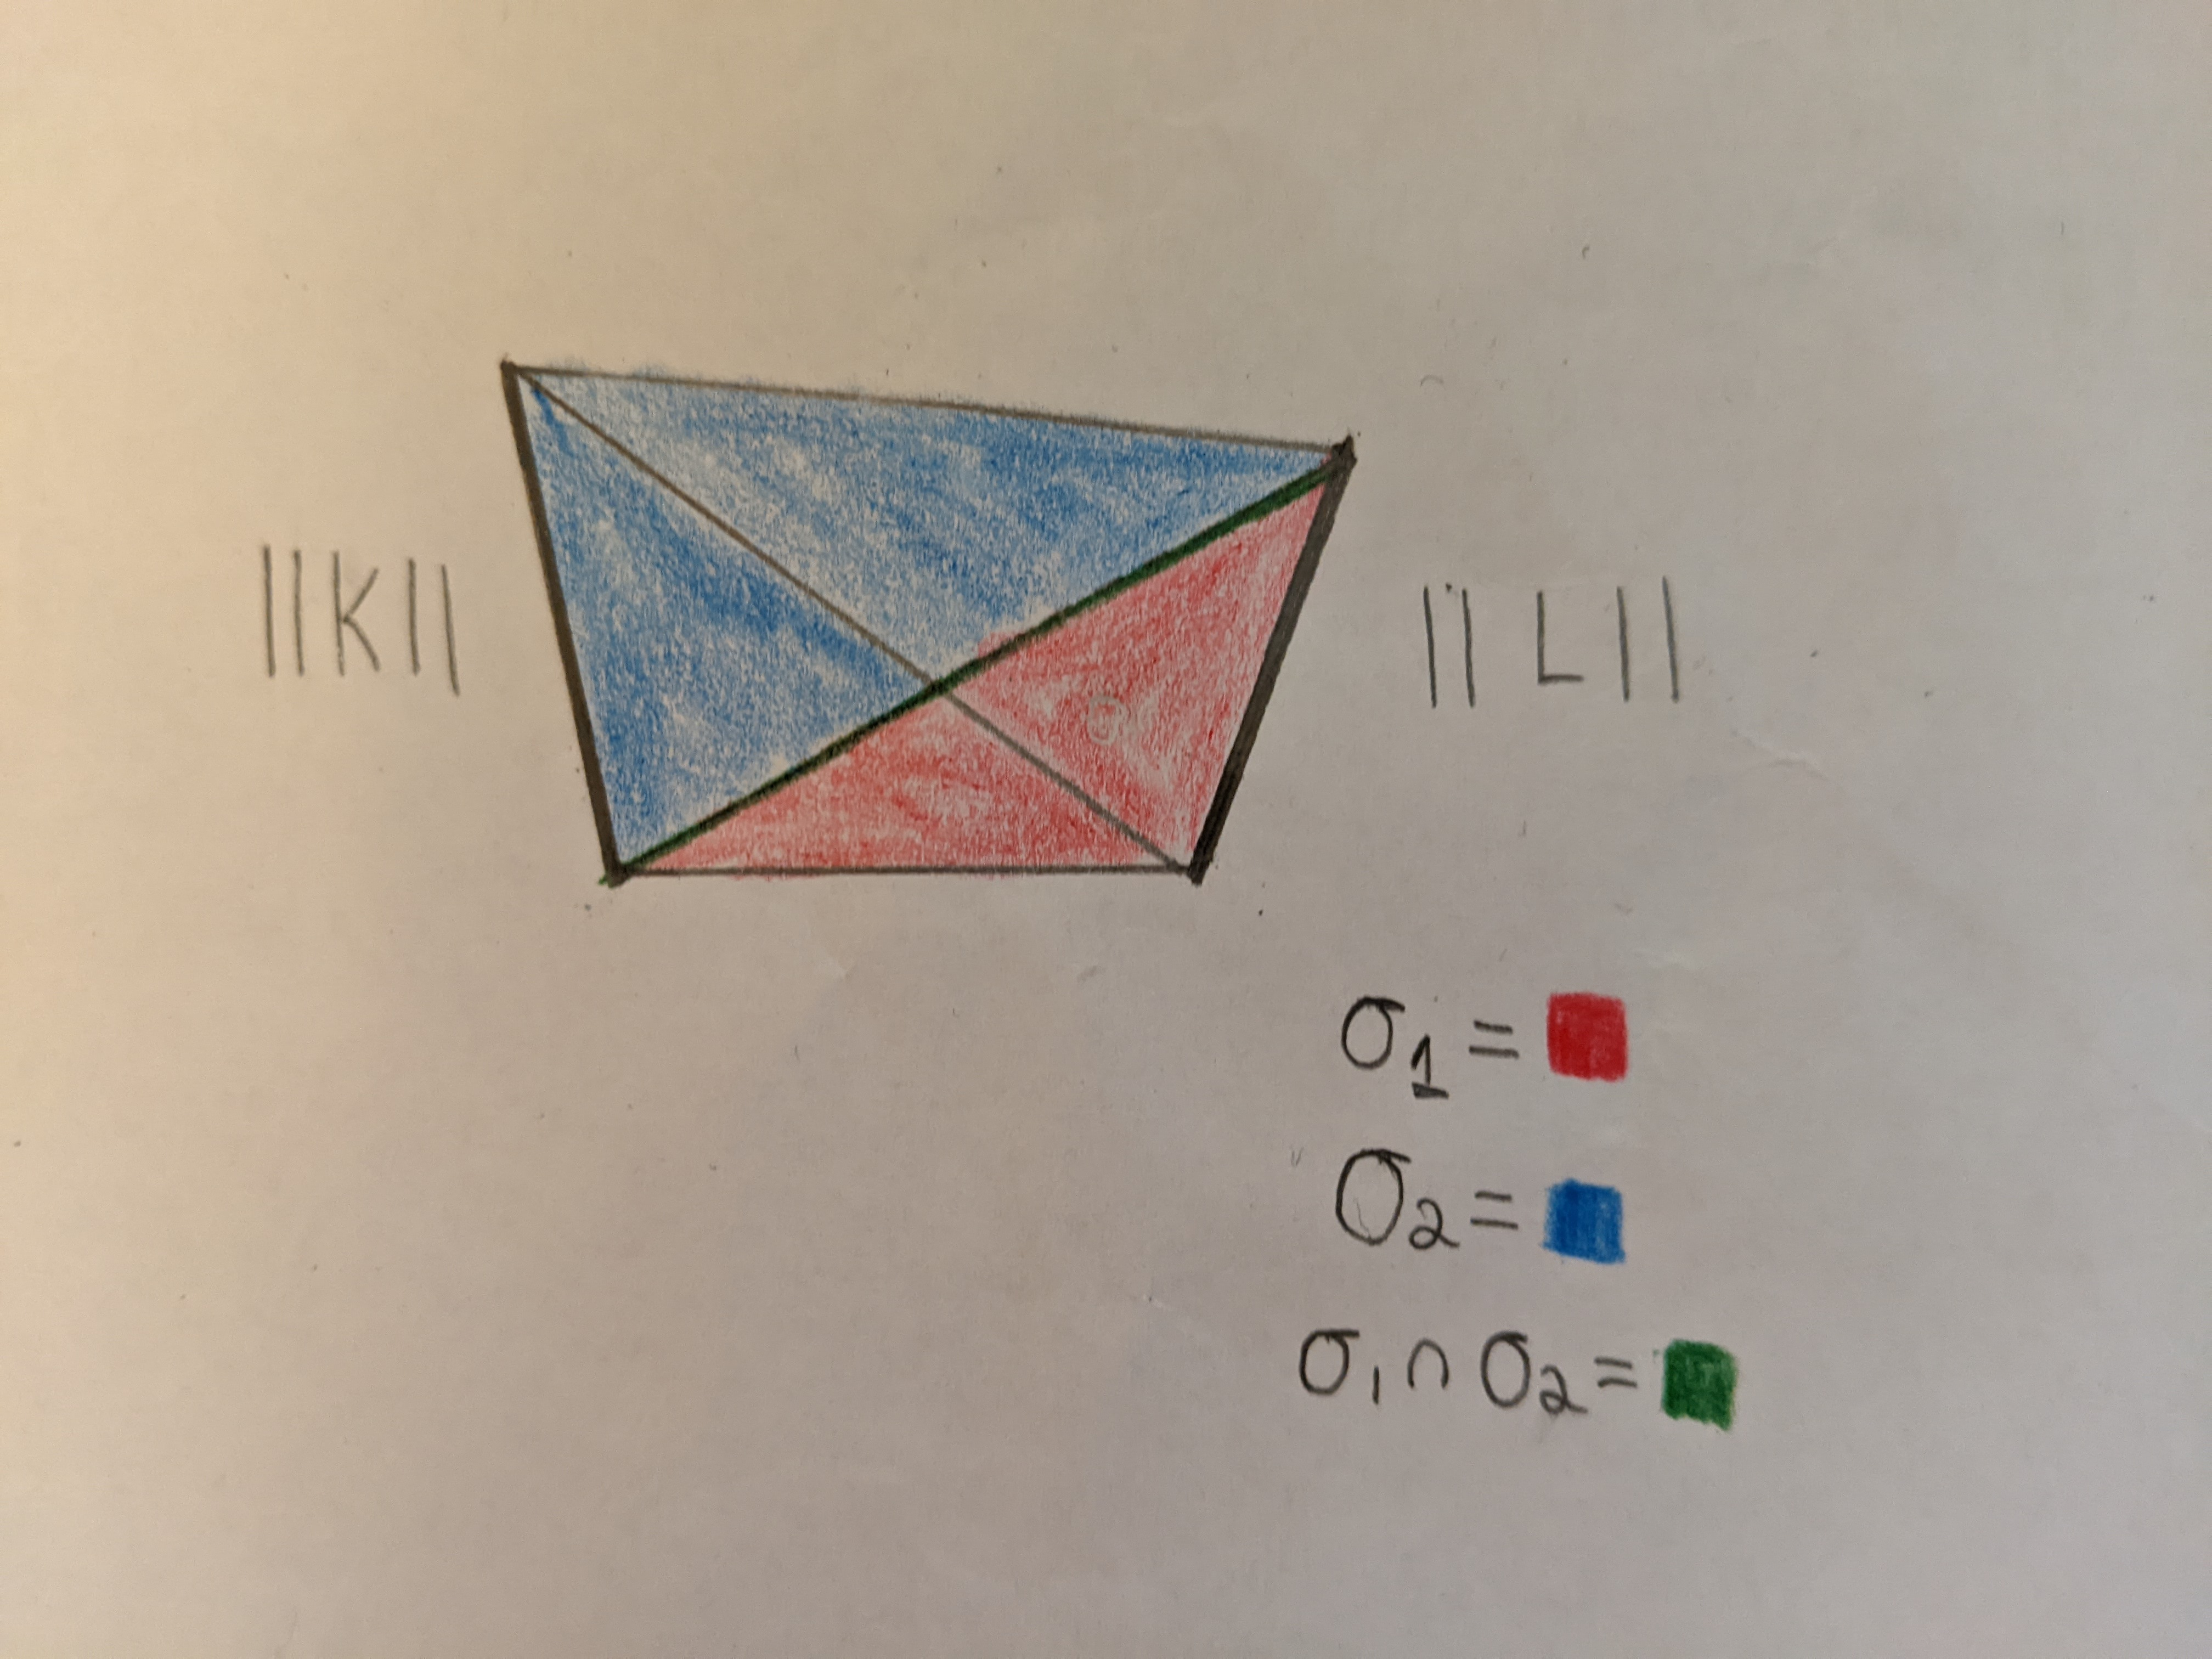
\includegraphics[width=\textwidth]{Image1}
\end{figure}
\newpage
\section*{Exercise 5.3.3}
\subsection*{Part A}
We construct a map $f: V_{n,2} \rightarrow S^{n-1}$ as follows:
\[
f(v_1,v_2) = \frac{v_1 + v_2}{\sqrt{2}}
\] Notice that
\[
f(-v_1,-v_2) = \frac{-v_1 -v_2}{\sqrt{2}} = -\frac{v_1+v_2}{\sqrt{2}} = -f(v_1,v_2)
\] Thus $f$ is a $\zz_2$-map from $V_{n,2}$ to $S^{n-1}$ so that $\text{ind}_{\zz_2}(V_{n,2}) \leq n - 1$.
\newpage
\subsection*{Part B}
We define a map $f: S^{n-1} \rightarrow V_{2,n}$ as follows:
\[
f(x_1,\ldots,x_n) = \big((x_1,\ldots,x_n),(-x_2,x_1,\ldots,-x_n,x_{n-1})\big)
\] (we can alternate signs in this manner because $n$ is even). We note that
\[
(x_1,\ldots,x_n) \cdot (-x_2,x_1,\ldots,-x_n,x_{n-1}) = x_1x_2 - x_1x_2 + \cdots - x_{n-1}x_n + x_{n-1}x_n = 0
\] so that $f$ does indeed map $S^{n-1}$ into $V_{2,n}$. Now, we note that
\begin{align*}
\nu(f(x_1,\ldots,x_n)) &= \nu\big((x_1,\ldots,x_n),(-x_2,x_1,\ldots,-x_n,x_{n-1})\big) \\
&= \big((-x_1,\ldots,-x_n),(x_2,-x_1,\ldots,x_n,-x_{n-1})\big)
\end{align*} and
\begin{align*}
f(-x_1,\ldots,-x_n) &= \big((-x_1,\ldots,-x_n),(x_2,-x_1,\ldots,x_n,-x_{n-1})\big)
\end{align*} so that $f$ is indeed a $\zz_2$-map from $S^{n-1}$ to $V_{2,n}$, thereby proving that $\text{ind}_{\zz_2}(V_{n,2}) = n - 1$ for $n$ even.
\newpage
\subsection*{Part C}
Suppose that $n$ is odd. Then $S^{n-2} \subseteq \rr^{n-1}$ and $n-1$ is even. We may define
\[
f(x_1,\ldots,x_{n-1}) = \big((x_1,\ldots,x_{n-1}),(-x_2,x_1,\ldots,-x_{n-1},x_{n-2})\big)
\] As above, we can show that
\[
\nu(f(x_1,\ldots,x_{n-1})) = \big((-x_1,\ldots,-x_{n-1}),(x_2,-x_1,\ldots,x_{n-1},-x_{n-2})\big) = f(-x_1,\ldots,-x_{n-1})
\] so that $f$ is a $\zz_2$-map from $S^{n-2}$ to $V_{2,n}$.
\newpage
\section*{Exercise 5.3.4} 
\subsection*{Part A}
We define $f: V_{2,n} \rightarrow V_{2,n}$ as follows:
\[
f(v_1,v_2) = \bigg(\frac{v_1+v_2}{\sqrt{2}}, \frac{v_1 - v_2}{\sqrt{2}}\bigg)
\] First, we note that
\[
\Vert v_1 + v_2 \Vert^2 = \langle v_1 + v_2, v_1 + v_2 \rangle = \langle v_1, v_1 \rangle + \langle v_1, v_2 \rangle + \langle v_2, v_1 \rangle + \langle v_2, v_2 \rangle = \Vert v_1 \Vert^2 + \Vert v_2 \Vert^2 = 2  
\] and that
\[
\Vert v_1 - v_2 \Vert^2 = \langle v_1 - v_2, v_1 - v_2 \rangle = \langle v_1, v_1 \rangle - \langle v_1, v_2 \rangle - \langle v_2, v_1 \rangle + \langle v_2, v_2 \rangle = \Vert v_1 \Vert^2 + \Vert v_2 \Vert^2 = 2  
\] because $v_1$ and $v_2$ are orthogonal. We obtain
\[
\Vert v_1 + v_2 \Vert = \Vert v_1 - v_2 \Vert = \sqrt{2}
\]
 Thus, we find that $f(v_1,v_2) \in (S^{n-1})^2$. Furthermore, we compute
\[
\bigg \langle \frac{v_1+v_2}{\sqrt{2}}, \frac{v_1 - v_2}{\sqrt{2}} \bigg \rangle = \frac{1}{2}(\langle v_1, v_1\rangle - \langle v_1, v_2 \rangle + \langle v_2, v_1 \rangle - \langle v_2, v_2 \rangle) = 0
\] so that $f$ does actually map $V_{2,n}$ into $V_{2,n}$. Now, we must show that $f \circ \omega_1 = \omega_2 \circ f$. Let $(v_1,v_2) \in V_{2,n}$. We compute
\[
f(\omega_1(v_1,v_2)) = f(v_2,v_1) = \bigg(\frac{v_1+v_2}{\sqrt{2}}, \frac{v_2 - v_1}{\sqrt{2}}\bigg)
\] and 
\[
\omega_2(f(v_1,v_2)) = \omega_2\bigg(\frac{v_1+v_2}{\sqrt{2}}, \frac{v_1 - v_2}{\sqrt{2}}\bigg) = \bigg(\frac{v_1+v_2}{\sqrt{2}}, \frac{v_2 - v_1}{\sqrt{2}}\bigg)
\] so that $f \circ \omega_1 = \omega_2 \circ f$. Thus, we find that $f$ is a $\zz_2$-map from $V_{2,n}$ to $V_{2,n}$. Now, we claim that $f^{-1} = f$. To see this, we compute
\begin{align*}
f(f(v_1,v_2)) = f\bigg(\frac{v_1+v_2}{\sqrt{2}}, \frac{v_2 - v_1}{\sqrt{2}}\bigg) = \Bigg(\frac{\frac{v_1+v_2}{\sqrt{2}} + \frac{v_1-v_2}{\sqrt{2}}}{\sqrt{2}}, \frac{\frac{v_1+v_2}{\sqrt{2}} - \frac{v_1-v_2}{\sqrt{2}}}{\sqrt{2}}\Bigg) = (v_1,v_2)
\end{align*} Thus, we find that $f$ is indeed its own inverse, so we only have to show that $f: (V_{2,n}, \omega_2) \rightarrow (V_{2,n},\omega_1)$ is a $\zz_2$-map. That is, we must show that $f \circ \omega_2 = \omega_1 \circ f$. Let $(v_1, v_2) \in V_{2,n}$. Then, we have
\[
f(\omega_2(v_1,v_2)) = f(v_1,-v_2) = \bigg(\frac{v_1 - v_2}{\sqrt{2}}, \frac{v_1+v_2}{\sqrt{2}}\bigg)
\] and
\[
\omega_1(f(v_1,v_2)) = \omega_1\bigg(\frac{v_1 + v_2}{\sqrt{2}}, \frac{v_1-v_2}{\sqrt{2}}\bigg) = \bigg(\frac{v_1 - v_2}{\sqrt{2}}, \frac{v_1+v_2}{\sqrt{2}}\bigg)
\] Thus we find that $f \circ \omega_2 = \omega_1 \circ f$ so that $f$ is a $\zz_2$-homeomorphism from $(V_{2,n},\omega_1)$ to $(V_{2,n},\omega_2)$.
\newpage
\subsection*{Part B}
First, we build a map $f: (V_{n,2}, \omega_1) \rightarrow (S^{n-1}, \nu)$ as follows:
\[
f(v_1,v_2) = \frac{v_1 - v_2}{\sqrt{2}}
\] We claim that $f \circ \omega_1 = \nu \circ f$. We compute
\[
f(\omega_1(v_1,v_2)) = f(v_2,v_1) = \frac{v_2 - v_1}{\sqrt{2}}
\] and
\[
\nu(f(v_1,v_2)) = \nu\bigg(\frac{v_1-v_2}{\sqrt{2}}\bigg) = \frac{v_2 - v_1}{\sqrt{2}}
\] so that $f \circ \omega_1 = \nu \circ f$. Thus we deduce that $\text{ind}_{\zz_2} (V_{n,2}) \leq n-1$. Next, we build a map $f: S^{n-2} \rightarrow V_{2,n}$ as follows:
\[
f(x_1,\ldots,x_{n-1}) = \big((0,\ldots,0,1), (x_1,\ldots,x_{n-1},0)\big)
\] Now, we claim that $\omega_2 \circ f = f \circ \nu$. Notice that
\[
f(\nu(x)) = f(-x) = f(-x_1,\ldots,-x_{n-1}) = \big((0,\ldots,0,1),(-x_1,\ldots,-x_{n-1},0)\big)
\] and that
\[
\omega_2(f(x)) = \omega_2\big((0,\ldots,0,1), (x_1,\ldots,x_{n-1},0)\big) = \big((0,\ldots,0,1),(-x_1,\ldots,-x_{n-1},0)\big)
\] Thus we find that $\omega_2 \circ f = f \circ \nu$ so that $f$ is a $\zz_2$-map and $n-2 \leq \text{ind}_{\zz_2}(V_{n,2})$.
\end{document} 